\section{Resultados de satisfação e desempenho da rede}
\paragraph{}
O questionário adotado para este trabalho foi o mesmo apresentado no curso de Administração e Gerência de Redes. O
questionário foi respondido por cinco usuários da rede:

\subsection{Desempenho da rede/Estabilidade da rede}

\noindent
\begin{minipage}{0.48\textwidth}
\centering
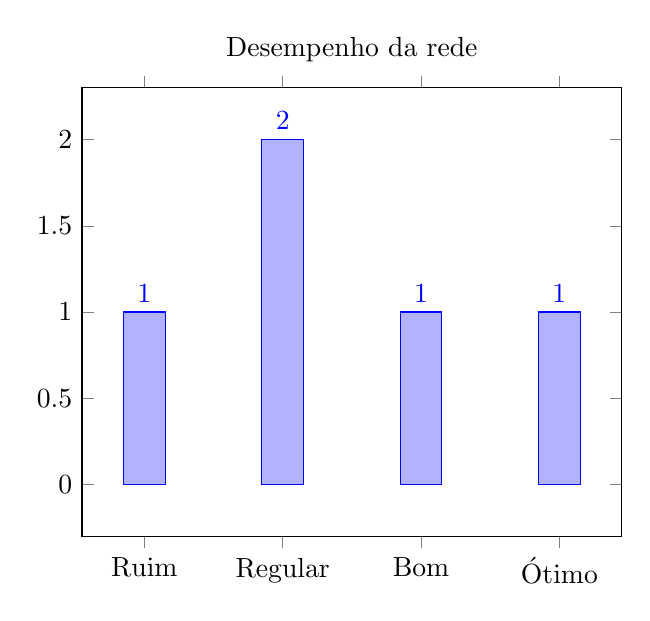
\begin{tikzpicture}
\begin{axis}[
    title={Desempenho da rede},
    ybar,
    bar width=15pt,
    enlargelimits=0.15,
    symbolic x coords={Ruim, Regular, Bom, Ótimo},
    xtick=data,
    nodes near coords,
    ymin=0,
]
\addplot coordinates {(Ruim, 1) (Regular, 2) (Bom, 1) (Ótimo, 1)};
\end{axis}
\end{tikzpicture}
\end{minipage}
\hfill
\begin{minipage}{0.48\textwidth}
\centering
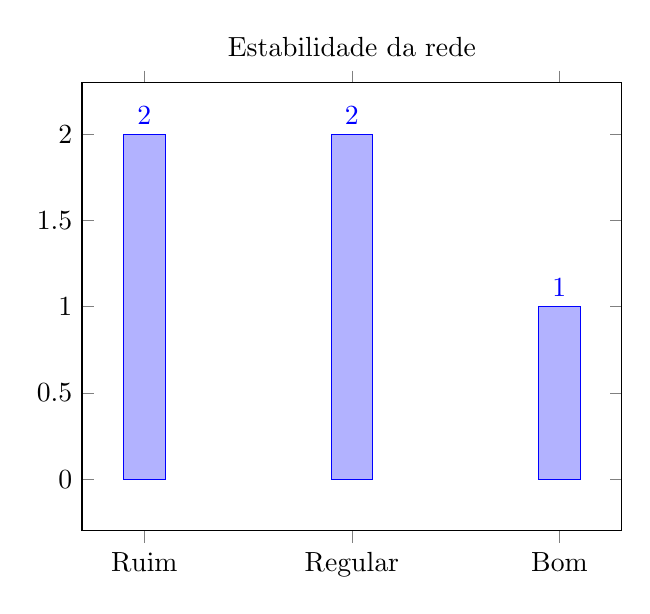
\begin{tikzpicture}
\begin{axis}[
    title={Estabilidade da rede},
    ybar,
    bar width=15pt,
    enlargelimits=0.15,
    symbolic x coords={Ruim, Regular, Bom},
    xtick=data,
    nodes near coords,
    ymin=0,
]
\addplot coordinates {(Ruim, 2) (Regular, 2) (Bom, 1)};
\end{axis}
\end{tikzpicture}
\end{minipage}

\subsection{Qualidade do suporte técnico/Tempo de resposta do suporte técnico}

\noindent
\begin{minipage}{0.48\textwidth}
\centering
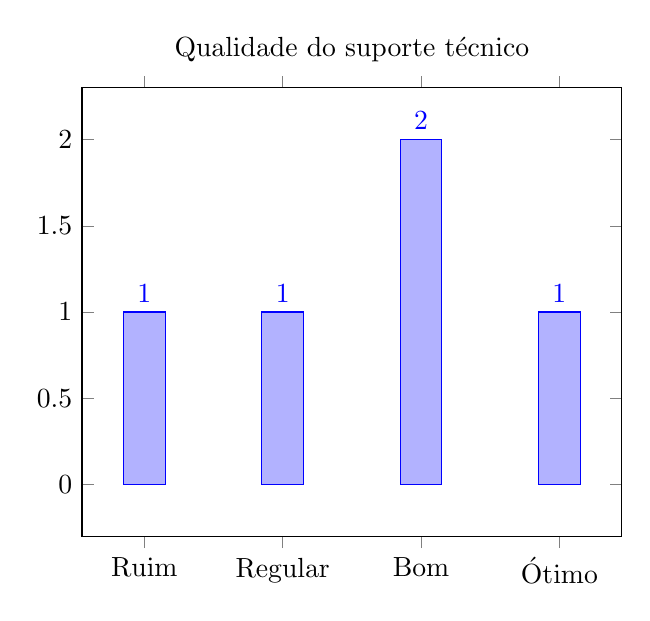
\begin{tikzpicture}
\begin{axis}[
    title={Qualidade do suporte técnico},
    ybar,
    bar width=15pt,
    enlargelimits=0.15,
    symbolic x coords={Ruim, Regular, Bom, Ótimo},
    xtick=data,
    nodes near coords,
    ymin=0,
]
\addplot coordinates {(Ruim, 1) (Regular, 1) (Bom, 2) (Ótimo, 1)};
\end{axis}
\end{tikzpicture}
\end{minipage}
\hfill
\begin{minipage}{0.48\textwidth}
\centering
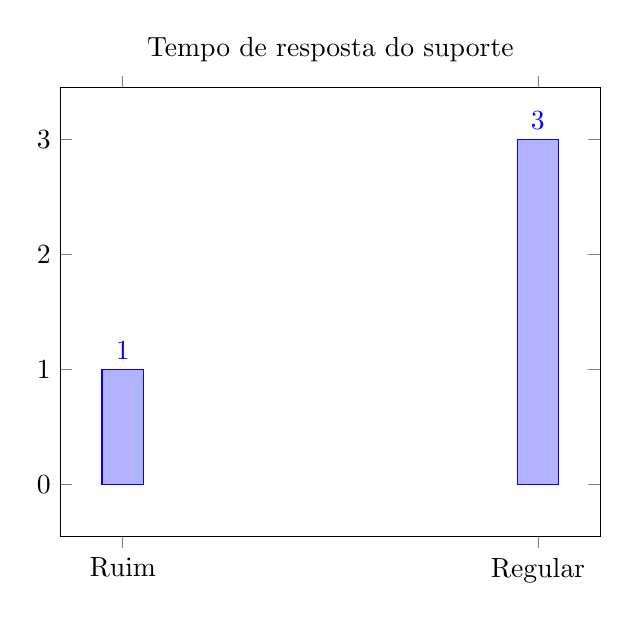
\begin{tikzpicture}
\begin{axis}[
    title={Tempo de resposta do suporte},
    ybar,
    bar width=15pt,
    enlargelimits=0.15,
    symbolic x coords={Ruim, Regular},
    xtick=data,
    nodes near coords,
    ymin=0,
]
\addplot coordinates {(Ruim, 1) (Regular, 3)};
\end{axis}
\end{tikzpicture}
\end{minipage}

\subsection{Qualidade de acesso à rede externa/ Qualidade dos serviços prestados}

\noindent
\begin{minipage}{0.48\textwidth}
\centering
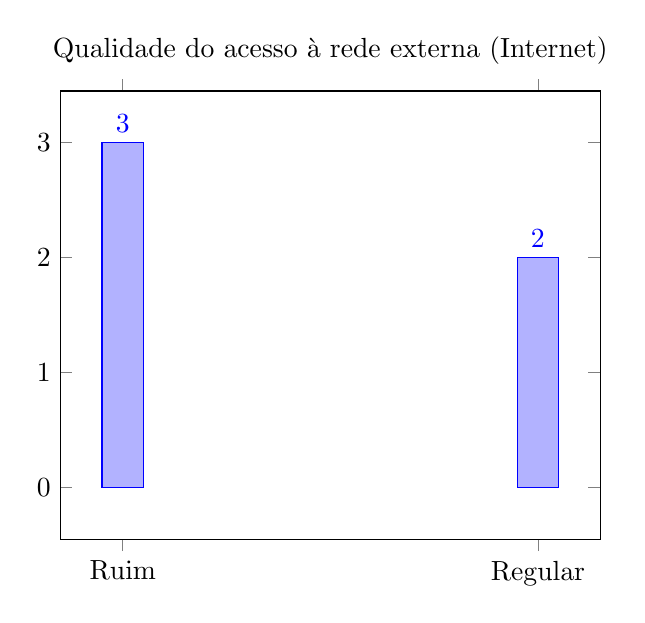
\begin{tikzpicture}
\begin{axis}[
    title={Qualidade do acesso à rede externa (Internet)},
    ybar,
    bar width=15pt,
    enlargelimits=0.15,
    symbolic x coords={Ruim, Regular},
    xtick=data,
    nodes near coords,
    ymin=0,
]
\addplot coordinates {(Ruim, 3) (Regular, 2)};
\end{axis}
\end{tikzpicture}
\end{minipage}
\hfill
\begin{minipage}{0.48\textwidth}
\centering
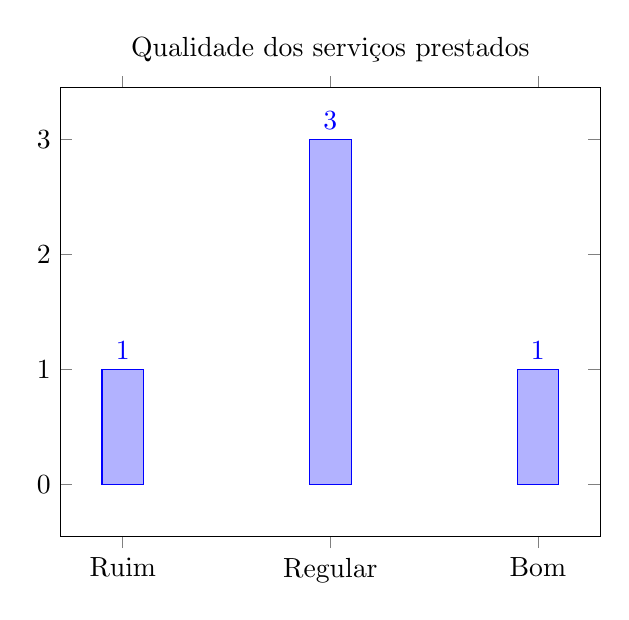
\begin{tikzpicture}
\begin{axis}[
    title={Qualidade dos serviços prestados},
    ybar,
    bar width=15pt,
    enlargelimits=0.15,
    symbolic x coords={Ruim, Regular, Bom},
    xtick=data,
    nodes near coords,
    ymin=0,
]
\addplot coordinates {(Ruim, 1) (Regular, 3) (Bom, 1)};
\end{axis}
\end{tikzpicture}
\end{minipage}

\subsection{Segurança de rede}

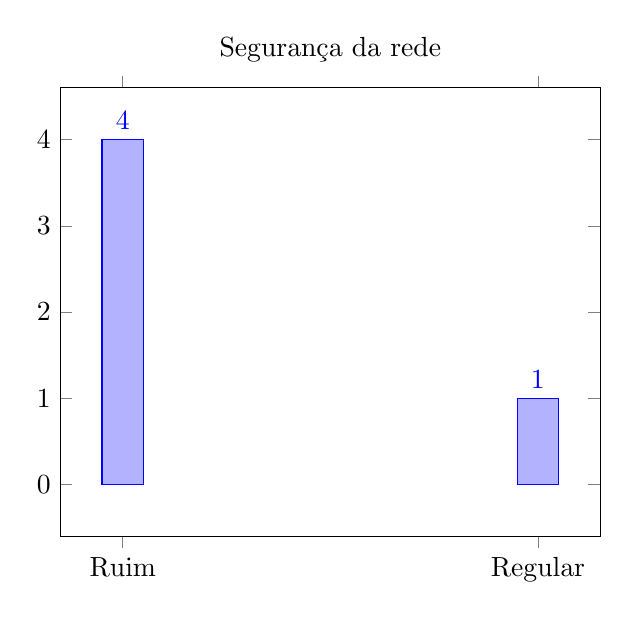
\begin{tikzpicture}
\begin{axis}[
    title={Segurança da rede},
    ybar,
    bar width=15pt,
    enlargelimits=0.15,
    symbolic x coords={Ruim, Regular},
    xtick=data,
    nodes near coords,
    ymin=0,
]
\addplot coordinates {(Ruim, 4) (Regular, 1)};
\end{axis}
\end{tikzpicture}
